\documentclass[conference]{IEEEtran}
\IEEEoverridecommandlockouts
% The preceding line is only needed to identify funding in the first footnote. If that is unneeded, please comment it out.
\usepackage{cite}
\usepackage{amsmath,amssymb,amsfonts}
\usepackage{algorithmic}
\usepackage{graphicx}
\usepackage{textcomp}
\usepackage{xcolor}
\usepackage{graphicx}
\usepackage{fancybox}
\usepackage[utf8]{inputenc}
\usepackage{epsfig,graphicx}
\usepackage{multicol,pst-plot}
\usepackage{pstricks}
\usepackage{amsmath}
\usepackage{amsfonts}
\usepackage{amssymb}
\usepackage{eucal}
\usepackage{subfigure}
\usepackage{enumitem}
\usepackage{hyperref}
\usepackage{algorithm}
\usepackage{algorithmic}

\def\BibTeX{{\rm B\kern-.05em{\sc i\kern-.025em b}\kern-.08em
    T\kern-.1667em\lower.7ex\hbox{E}\kern-.125emX}}
\begin{document}

\title{ECE276B Project 1: Dynamic Programming}

\author{\IEEEauthorblockN{Awies Mohammad Mulla}
\IEEEauthorblockA{ MS ECE\\
ISRC\\
A59016119\\
amulla@ucsd.edu}
}

\maketitle
\begin{abstract}

\end{abstract}

\section{Introduction}
We are implementing a dynamic programming algorithm to find the optimal path for a robot to traverse a grid. The problem is formulated as a Markov Decision Process (MDP). The actions of the robot comprises of simple actions: forward step, turn right, turn left and special actions: picking-up the key and unlocking the door. Since, the status of the door could be both open and close, our optimal policy will differ accordingly (whether to pick up the key for opening the door or not) and it is this fact which make this problem more challenging compared to solving a simple 2D grid. \\
The problem of Optimal Control is an essential area of research in robotics which is linked to every field of robotics. From autonomous cars in the form of motion planning to robotic arms in the form of trajectory planning, the problem of optimal control is ubiquitous. The current project is form of an optimal control (motion planning) problem on a much smaller scale. It can be explained as a robot trying to find the optimal path to reach a goal state from a start state. The robot has to avoid obstacles and depending on the state of the door robot has to pick up the key which is somewhat similar to traversing through a waypoint. \\
We are solving the mentioned problem using Forward Dynamic Programming. We have formulated the problem as a Markov Decision Process (MDP) in the form of non-directional graph in which the nodes consists of the state of the robot mentioned in the Problem Formulation and the edges representing the costs of traversing between nodes. The connectivity of the nodes is further described in the Formulation and the cost on edges here has been taken as equal for all edges. Using Dynamic Programming we are traversing through the graph to find the optimal path (to each of the nodes progressively).
\section{Problem Formulation}
The problem is formulated as a MDP i.e., the next state of the system is only dependent on the current state and the input provided at that timestep. The state of the system consists of pose of the agent (position and direction), status of the key with the agent (whether the agent has picked up the key or not) and the status of the door (whether the door is open or closed). The input to the system is the action taken by the agent at that timestep. The actions are simple actions: forward step, turn right, turn left and special actions: picking-up the key and unlocking the door. The elements of the MDP are defined below:
\begin{itemize}
\item \textbf{State Space}: The state space ($\chi$) consists of all the possible states ($x$) of the system. The state of the system is defined as $x = [x_1, x_2, x_3, x_4, x_5, x_6]^T$. The elements of the state vector are defined as follows:
\begin{align*}
x_1 &= \text{X-coordinate of the agent in the grid}\\
x_2 &= \text{Y-coordinate of the agent in the grid}\\
x_3 &= \text{Direction of the agent in the grid along x-axis}\\
x_4 &= \text{Direction of the agent in the grid along y-axis}\\
x_5 &= \text{Status of the key with the agent (0: No, 1: Yes)}\\
x_6 &= \text{Status of the door (0: Closed, 1: Open)}
\end{align*}
where $x_1, x_2 \in \mathbb{W}$; $\mathbb{W}$ is the set of all the possible coordinates in the grid and $x_3, x_4 \in \{-1, 0, 1\}$.
\item \textbf{Control Space}: The control space ($\mathbb{U}$) consists of all the possible actions ($u \in $ {Forward (MF), Turn Right (TR), Turn Left (TL), Pick Key (PK), Unlock Door (UD)}) that the agent can take. We can defined the actions as follows (to suit our motion model):
\begin{align*}
u &=[1 \ 0 \ 0 \ 0 \ 0] \text{Forward Step}\\
u &=[1 \ 0 \ 0 \ -1 \ -1] \text{Turn Right}\\
u &=[0 \ 0 \ 0 \ 1 \ -1] \text{Turn Left}\\
u &=[0 \ 1 \ 0 \ 0 \ 0] \text{Pick-up Key}\\
u &=[0 \ 0 \ 1 \ 0 \ 0] \text{Unlock Door}
\end{align*}
\item \textbf{Motion model}: The motion model ($f$) describes the dynamics of the system. The motion model is defined as follows:
\begin{equation*}
    x_{t+1} = x_{t} + Bu_t
\end{equation*}
where $x_t$ is the state of the system at time $t$ and $u_t$ is the action taken by the agent at time $t$. we get above motion model since we know no noise is present in the system. The matrix $B$ is defined as follows:
\begin{equation*}
    B = \begin{bmatrix}
    x_3 & 0 & 0 & 0 & 0 & 0\\
    0 & x_4 & 0 & 0 & 0 & 0\\
    0 & 0 & 0 & 0 & x_4 & x_3\\
    0 & 0 & 0 & 0 & x_3 & x_4\\
    0 & 1 & 0 & 0 & 0 & 0\\
    0 & 0 & 1 & 0 & 0 & 0
    \end{bmatrix}
\end{equation*}
\item \textbf{Initial State}: The initial state of the system comprise of agent position and direction in the format mentioned above along with the status of the key and the door (both 0).
\item \textbf{Planning Horizon}: The planning horizon ($T$) is the maximum number of timesteps for which the agent has to plan the optimal path. Here it would be simply be taken as total number of nodes in the graph, for instance in the case of 5x5 grid it would be (5x5x4x2=200; 2 is for status of key).
\item \textbf{Cost Function}: The cost function ($c$) is the function which defines the cost of taking an action at a particular state. The cost function is defined as $c=1$ for all the actions.
\end{itemize}

\section{Technical Approach}
The problem is solved using Forward Dynamic Programming. To obtain optimal action sequence we are first calculating the cost to reach each state (and goal state). The algorithm to calculate costs-to-go is described below:
\begin{itemize}
\item Initialize the cost to reach each state as $\infty$ except the start state which is 0.
\item Initialize an open list (this will contain the state as well as action to be taken at that state) which contains the states to be explored.
\item Now insert the start state with possible actions at that state (TR, TL, MF, PK, UD) into the open list.
\item Loop till the open list is empty or planning horizon is reached.
\item During each loop, pop the first element from the open list and calculate the cost to reach the state which we will obtain on applying the popped input to the system with popped state using following equation:
\begin{equation*}
    V_{t+1}(x_{t+1}) = \min \{c(x_t, u_t) + V_t(x_t), V_t(x_t)\}
\end{equation*}
where, $V_t(x_t)$ is the cost to reach the state $x_t$ at time $t$ and $V_{t+1}(x_{t+1})$ is the cost to reach the state $x_{t+1}$ at time $t+1$. The cost function $c(x_t, u_t)$ is defined above.
\item If the cost-to-go of a particular state is updated, then insert the state with possible actions at that state into the open list. If it is not updated i.e., the cost becomes stationary ($V_{t+1}(x_{t+1})=V_t(x_t)$) then do not insert the state into the open list as this will be final cost-to-go for that state.
\item We will loop till the open list is empty or planning horizon is reached.
\end{itemize}
After finding the cost-to-go for each state, we will find the optimal action sequence by backtracking from the goal state to the start state, using the cost table. This algorithm essentially requires the connectivity of the graph to be known beforehand (which was used to formulated the Motion model of the MDP).

\section{Results}

\subsection{Grids}
\begin{figure}[H]
\centering
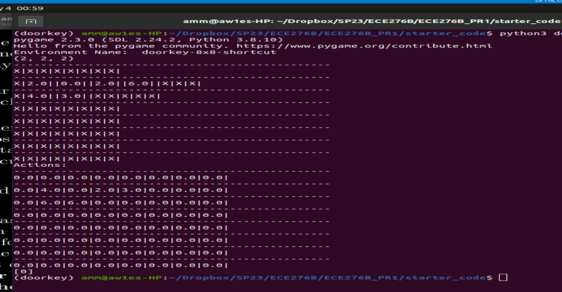
\includegraphics[width=0.8\textwidth]{8x8_grid.png}
\caption{8x8 Grid}
\end{figure}


\subsection{Analysis}
\begin{itemize}
\item We were able to find the optimal cost-to-go for each state in the grid for all the grids in the known environment.
\item Due to lack of time we were not able to implement the algorithm for the unknown environment.
\item The results mentioned above are the images of the cost-to-go grids with minimum costs at each coordinate (among all directions).
\item We could have been able to extract the optimal action sequence from the cost-to-go grid, but due to lack of time we were not able to implement it.
\item The algorithm would be straightforward depending upon difference in the cost-to-go values and states.
\end{itemize}

\end{document}
